\subsection{Random Forest (Rừng ngẫu nhiên)}
    \label{label:rf}
    \subsubsection{Khái niệm: Bootstrapping và Bagging}
    
    Bootstrapping là một phương pháp nổi tiếng trong thống kê được giới thiệu bởi Bradley Efron vào năm 1979 \cite{efron1992bootstrap}. Phương pháp này thực hiện lặp lại nhiều lần:
        \begin{itemize}
            \item Lấy ra một mẫu có hoàn lại từ mẫu ban đầu
            \item Ước tính các tham số mong muốn từ mẫu lấy được
        \end{itemize}
    Từ đó, ước lượng được các tham số mong muốn từ mẫu ban đầu. Phương pháp này chủ yếu dùng để ước lượng lỗi chuẩn (standard errors), độ lệch (bias) và tính toán khoảng tin cậy (confidence interval) cho các tham số.
    
    Bootstrap Aggregating (Bagging) là thuật toán kết hợp các mô hình máy học. Thuật toán sử dụng phương pháp Bootstrap để tạo nhiều bộ dữ liệu đầu vào từ một bộ dữ liệu, sau đó xây dựng các độc lập mô hình có cùng thuật toán nhưng với từng bộ dữ liệu đầu vào khác nhau. Các mô hình này sẽ được kết hợp bằng phương pháp biểu quyết đa số (majority voting).

    \begin{figure}[htp]
        \centering
        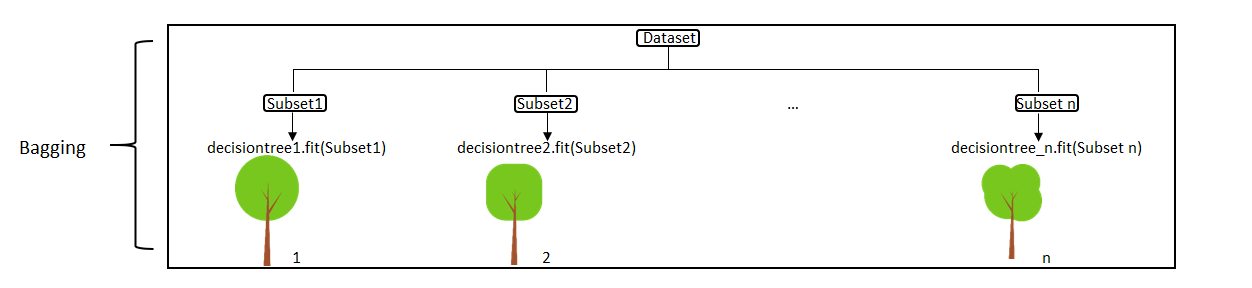
\includegraphics[width=16 cm]{images/bagging.png}
        \caption{Minh họa: Bagging}
        \label{fig:bagging}
    \end{figure}
    
    \subsubsection{Khái niệm: Random Forest}
    
    Random Forest \cite{breiman2001random}, hay còn gọi là Random Decision Forest, là một phương pháp ensemble, kết hợp nhiều mô hình cây quyết định phân lớp/hồi quy (Classification and regression trees - CART), cải tiến của phương pháp Bagging. RF được phát triển bởi Leo Breiman. Ông đồng thời cũng là tác giả của CART \cite{breiman_1984}
    
    \subsubsection{Mô tả thuật toán xây dựng Random Forest}
    
    \begin{itemize}
        \item Bước 1: Chọn ngẫu nhiên k từ n thuộc tính (k<n) có trong bộ dữ liệu huấn luyện.
        
        \item Bước 2: Sử dụng phương pháp boostrapping, chọn có hoàn lại từ bộ dữ liệu huấn luyện để tạo ra một bộ dữ liệu mới.
        
        \item Bước 3: Xây dựng cây quyết định với bộ dữ liệu ở bước 2, chỉ sử dụng k thuộc tính đã chọn ở bước 1
        
        \item Bước 4: Lặp lại Bước 2-3 để tạo nhiều cây quyết định khác.
        
        \item Bước 5: Kết hợp các cây quyết định thành phần bằng phương pháp bỏ phiếu.
    \end{itemize}
    
    \begin{figure}[htp]
        \centering
        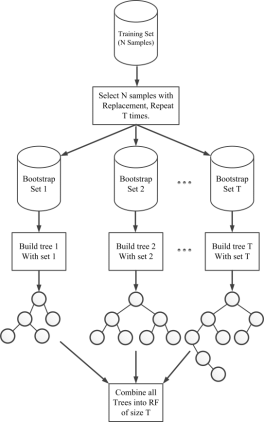
\includegraphics[width=8 cm, height=10cm]{images/Structure-of-random-forest.png}
        \caption{Minh họa: Random Forest \cite{RF_structure}}
        \label{fig:RF}
    \end{figure}
    
    \subsubsection{Dự đoán bằng Random Forest}
    
    Với x là một điểm dữ liệu mới, mỗi cây thành phần dự đoán hồi quy $T_{i}(x)$, dự đoán hồi quy của mô hình là:
    \begin{equation} \label{RF_reg}
        \hat{f}^{N}_{rf}(x) = \frac{1}{N} \underset{i=1}{ \overset{N}{\Sigma}} T_{i}(x)
    \end{equation}
    
    Với  $\hat{T}_{i}(x)$ là kết quả phân lớp của cây thành phần, dự đoán phân lớp của mô hình là:
    \begin{equation} \label{RF_cls}
        \hat{C}^{N}_{rf}(x) = majority \: vote \: \{\hat{T}_{i}(x)\}^{N}_{1}
    \end{equation}
    
    \subsubsection{Đánh giá Random Forest}
    
    Do sử dụng phương pháp boostrapping để tạo các mẫu huấn luyện cho các CART thành phần, chỉ có khoảng $\frac{2}{3}$ dữ liệu không trùng lặp trong bộ huấn luyện ban đầu được sử dụng cho việc huấn luyện. $\frac{1}{3}$ dữ liệu còn lại không tham gia huấn luyện được gọi là 'Out-of-bag dataset' (OOB). Phần dữ liệu này có thể xem như là một tập kiểm thử (validation dataset) dùng để đánh giá và tính toán độ quan trọng các thuộc tính của các CART trong rừng. Độ lỗi của RF trên tập dữ liệu OOB được gọi là 'Out-of-bag Error' ($E_{OOB}$).
    
    \begin{figure}[htp]
        \centering
        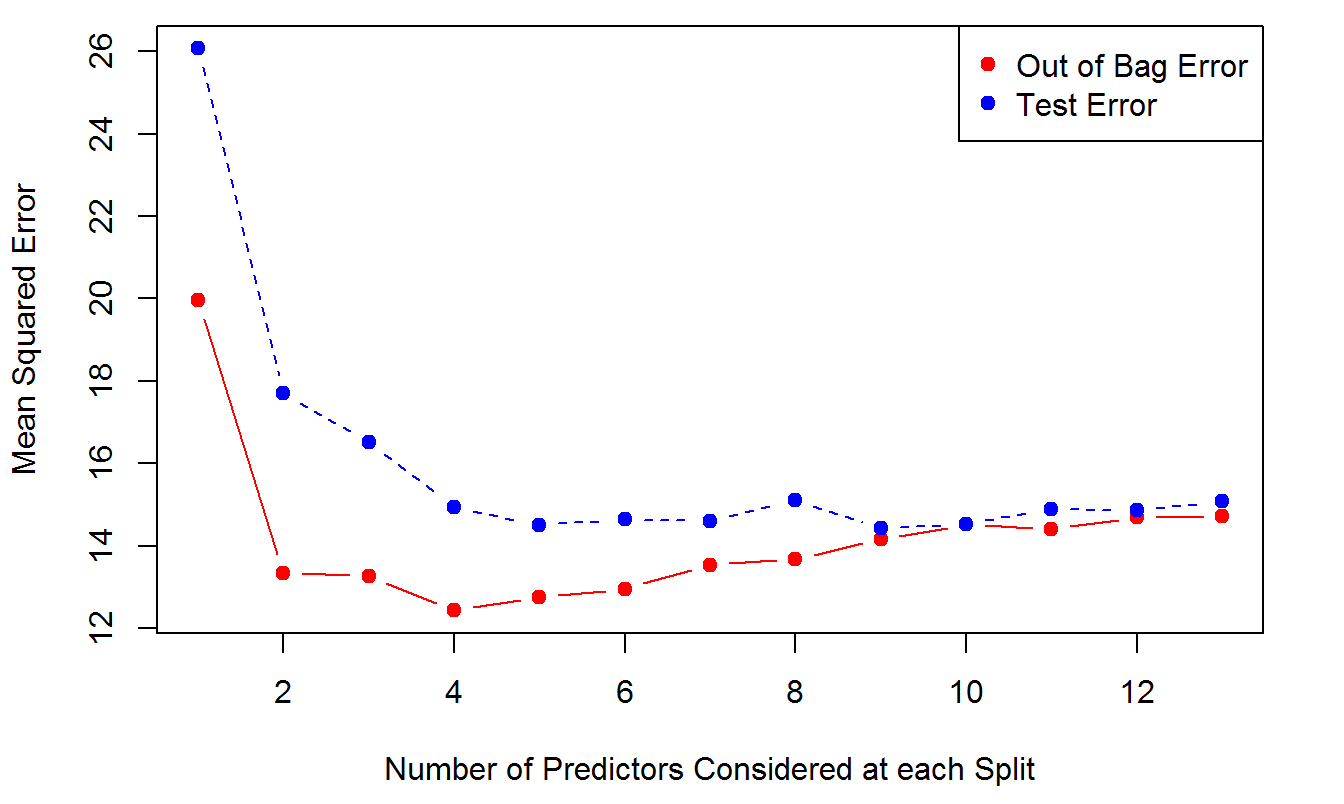
\includegraphics[width=12 cm]{images/rf_oob.png}
        \caption{Tương quan Out-of-bag error và test error}
        \label{fig:RF}
    \end{figure}
    
    Có thể so sánh $E_{OOB}$ giữa các RF có số thuộc tính được chọn k (ở bước 1) khác nhau và số lượng cây trong rừng khác nhau để chọn được mô hình RF có độ lỗi thấp nhất. 
    
    \subsubsection{Điểm mạnh của Random Forest}
    
    Thuật toán xây dựng có sự ngẫu nhiên trong mẫu dữ liệu (dùng phương pháp bootstrapping) và ngẫu nhiên trong số thuộc tính của mẫu so với tập thuộc tính ban đầu. Do đó, các tập huấn luyện con được tạo ra có tính đa dạng, ít liên quan. Mỗi CART xây dựng từ những tập dữ liệu con này không dùng tất cả dữ liệu training, cũng như không dùng tất cả các thuộc tính của dữ liệu để xây dựng nên mỗi cây có bias cao. Tuy nhiên, kết quả cuối của RF là kết hợp của nhiều cây thành phần, thông tin từ các cây sẽ bổ sung thông tin cho nhau, dẫn đến mô hình có low bias và low variance, tức là mô hình có kết quả dự đoán tốt.
    
    Trong rừng, mỗi cây thành phần chỉ được huấn luyện trên một tập nhỏ các thuộc tính thay vì toàn bộ (bước 1), cơ chế này giúp RF thực thi nhanh khi áp dụng trên tập dữ liệu có số lượng lớn thuộc tính. Hơn nữa, việc xây dựng từng cây thành phần là độc lập nên có thể dễ dàng thực hiện song song.


\subsection{Gradient Boosting (Tăng cường độ dốc)}
    \subsubsection{Khái niệm: Boosting}
        Boosting là một kỹ thuật ensemble với mục đích từ một số mô hình học yếu (weak learner) tạo ra mô hình học mạnh hơn (strong learner) bằng cách cho những mô hình sau sửa lỗi (học từ lỗi) của các mô hình trước. Các mô hình được thêm vào theo cách này cho đến khi đạt số lượng mô hình tối đa cho phép hoặc dự đoán hoàn toàn trùng khớp với tập huấn luyện.
        
        \begin{figure}[htp]
            \centering
            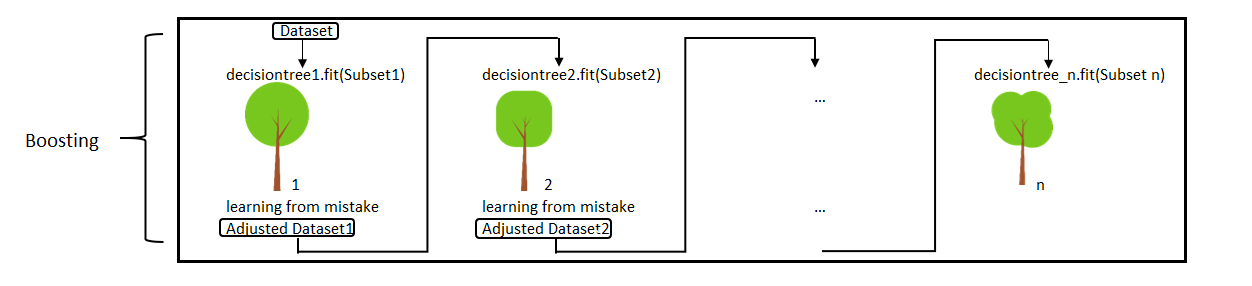
\includegraphics[width=16cm]{images/boosting.png}
            \caption{Minh họa: Boosting}
            \label{fig:boosting}
        \end{figure}
        
        Thuật toán boosting đơn giản nhất là Ada Boost, được giới thiệu vào năm 1995 bởi Freund và Schapire \cite{freund1997decision}.
        Thuật toán này sử dụng các CART có độ sâu nhỏ, hay còn gọi là một gốc (stump), làm các weak learner thành phần. 
        
        Ada Boost thực hiện việc học tăng cường bằng cách gán cho mỗi điểm dữ liệu trong bộ huấn luyện bộ huấn luyện một trọng số mẫu (sample wieght). Ban đầu, tất cả điểm dữ liệu đều được khởi tạo trọng số này bằng $\frac{1}{n}$, với n là tổng số điểm dữ liệu. Sau đó, với mỗi gốc được tạo, tổng lỗi của gốc đó sẽ quyết định trọng số của gốc trong việc bỏ phiếu (wieghted voting) cho kết quả dự đoán cuối. Những điểm dữ liệu cũng được cập nhật lại sample wieght dựa vào kết quả gốc hiện tại dự đoán đúng (sample wieght giảm) hay dự đoán sai (sample wieght tăng) thể hiện gốc sau đó cần dự thiết dự đoán đúng các điểm dữ liệu đang được dự đoán sai (gốc tiếp theo cố gắng sửa lỗi của gốc trước đó)
        
        Cụ thể thuật toán Ada Boost như sau \cite{freund1999short}:
        \begin{itemize}
            \item Khởi tạo $w_{1} = \{\frac{1}{N}\}^{N}_{1}$
            
            \item Với M là số gốc tối đa, lặp lại m=1,...M:
            \begin{itemize}
                \item Huấn luyện gốc sử dụng sample weight $w_{m}$
                
                \item Tính độ lỗi: 
                \begin{equation}
                    \epsilon_{t} = Pr_{i~D_{t}} [ h_{t} \ne y_{i} ]
                \end{equation}
                
                \item Thiết lập trọng số cho gốc này:
                    \begin{equation}
                        \alpha_{t} = \frac{1}{2}\ln{\frac{1 - \epsilon_{t}}{\epsilon_{t}}}
                    \end{equation}
                
                \item Cập nhật sample wieght cho việc huấn luyện gốc tiếp theo:
                    \begin{equation}
                        D_{t+1} = \frac{D_{t}(i)e^{-\alpha_{t}}}
                        {Z_{t}}
                    \end{equation}

                (với $Z_{t}$ là hệ số chuẩn hóa để tổng sample wieght bằng 1)
                
            \end{itemize}
            
            \item Cuối cùng, kết hợp các gốc bằng bỏ phiếu có trọng số:
                \begin{equation}
                    H(x) = sign( \underset{t=1}{ \overset{T}{\Sigma}} \alpha_{t} h_{t}(x) )
                \end{equation}
                \vspace{0.5cm}
    \clearpage
        \end{itemize}
        \clearpage
        \begin{figure}[H]
        \centering
        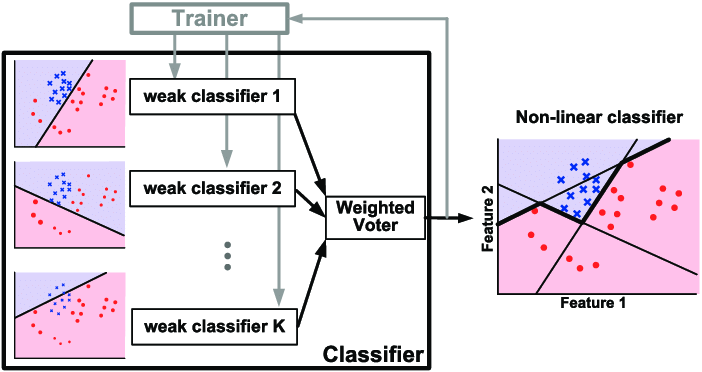
\includegraphics[width=8.5 cm,]{images/adaboost.png}
        \caption{Minh họa thuật toán AdaBoost, quá trình kết hợp các mô hình yếu \cite{adab_pic}}
        \label{fig:adab}
        \end{figure}
        
        
    \subsubsection{Gradient Boosting}
        Ý tưởng của thuật toán Gradient Boosting (GB) bắt nguồn từ Leo Breiman. Ông cho rằng phương pháp boosting có thể xem như là một thuật toán tối ưu hóa trên một hàm mất mát (Loss function) phù hợp \cite{breiman1997arcing}. Thuật toán Gradient boosting sau đó được phát triển bởi Jerome H. Friedman \cite{friedman2001greedy} \cite{friedman2002stochastic}.
        
        Khác với Ada Boost, ở Gradient Boosting:
            \begin{itemize}
                \item Sử dụng cây phân lớp, hồi quy làm các weaker learner thành phần thay vì gốc
            
                \item Những CART thành phần không huấn luyện dựa trên trọng số mẫu (mô hình tiếp theo cố gắng dự đoán đúng những điểm lỗi của mô hình trước), mà dựa trên  'độ lệch (lỗi) giả'(pseudo-residual) của CART tiền nhiệm trước đó (mô hình tiếp theo cố gắng giảm độ lỗi có được từ mô hình trước).
                
                \item Những mô hình thành phần không có trọng số riêng, thay vào đó chúng có chung một tỉ lệ tốc độ học (learning rate) trong khoảng {0-1} để điều chỉnh tốc độ học của từng mô hình mới.
            \end{itemize}
            
        Thuật toán kết thúc khi đạt số lượng cây tối đa hoặc việc thêm những cây mới không giảm pseudo-residual.
            
        \begin{figure}[htp]
        \centering
        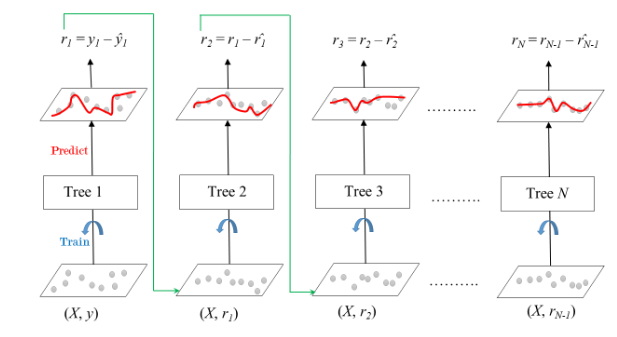
\includegraphics[width=10 cm,]{images/gradientboosting.png}
        \caption{Minh họa: Gradient boosting \cite{g4g_Gb}}
        \label{fig:gb}
        \end{figure}

        
    \subsubsection{Thuật toán Gradient Boosting \cite{starmer_2019_GBR} \cite{starmer_2019_GBC}:}
        
        Input: Dữ liệu huấn luyện $ \{(x_{i}, y_{i})\}^{n}_{i=1} $, một hàm Loss $ L(y, F(x)) $ và số lượng cây tối đa M
        \begin{itemize}
            \item Bước 1: Khởi tạo dự đoán ban đầu với hằng số
                \begin{equation}
                    F_{0}(x) = \underset{\gamma}{\mathrm{argmin}} \, 
                    \underset{i=1}{ \overset{n}{\Sigma}} L(y_{i}, \gamma)
                \end{equation}

            \item Bước 2: Lặp m=1 đến M để tạo M cây thành phần:
                \begin{description}
                    \item (A) Tính 'độ lệch giả' (pseudo-residual) của các điểm dữ liệu trong tập huấn luyện: Với mỗi i = 1, ..., n
                        \begin{equation}
                            r_{im} = -[\frac{\partial L(y_{i}, F(x_{i}))} {\partial F(x_{i})}]_{F(x) = F_{m-1}(x)}
                        \end{equation}
                        
                    \item (B) Xây dựng cây dự đoán các giá trị $r_{im}$, gọi $R_{jm}$ là các lá của cây, vớij=1, ...,$J_{m}$ (cây có $J_{m}$ lá)
                    
                    \item (C) Tính giá trị output ở từng lá của cây vừa tạo :
                        \begin{equation}
                            \gamma_{jm} = \underset{\gamma}{\mathrm{argmin}} \, 
                            \underset{x_{i} \in R_{ij}}{\Sigma}
                            L(y_{i}, F_{m-1}(x_{i}) + \gamma)
                        \end{equation}
                        
                    \item (D) Cập nhật dự đoán mới:
                        \begin{equation}
                            F_{m}(x) = F_{m-1}(x) + \nu \underset{j=1}{\overset{J_{m}}{\Sigma}}
                            \gamma_{m} I(x \in R{jm})
                        \end{equation}
                        với $\nu$ là tỷ lệ tốc độ học (learning rate)
                    
                \end{description}
                
        \end{itemize}
        
        Output: Kết quả dự đoán là kết quả của cây cuối cùng: $F_{M}(x)$
        
    \subsubsection{Điểm mạnh của Gradient Boosting}
        Qua mỗi cây mới được thêm vào, độ lỗi của mô hình sẽ ngày càng được giảm. Với các siêu tham số (hyperparameter) hợp lý, mô hình có thể cho được độ chính xác cao.
        
        \begin{figure}[htp]
        \centering
        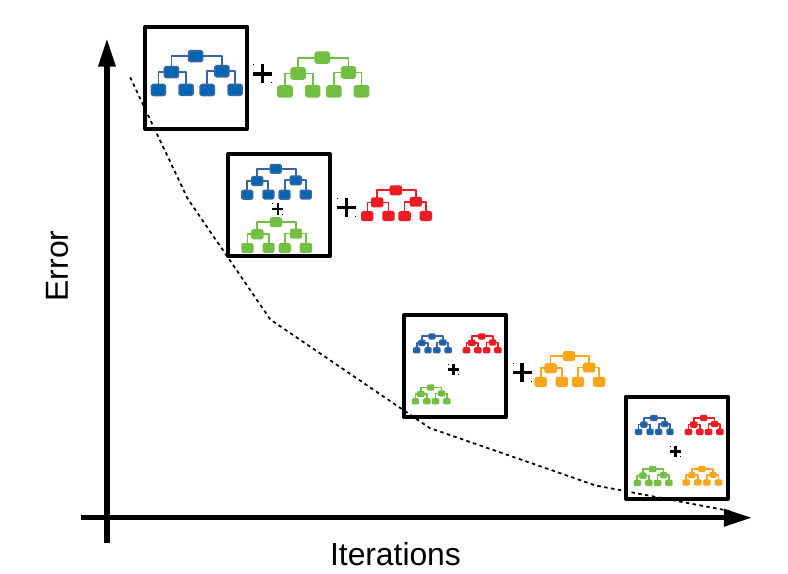
\includegraphics[width=10 cm,]{images/GB_error.png}
        \caption{Độ lỗi qua các iteration - GB \cite{gb_graph}}
        \label{fig:gb}
        \end{figure}
            
        Gradient Boosting có thể được tối ưu với nhiều hàm Loss khác nhau và cho phép hiệu chỉnh (fine tunning) nhiều siêu tham số (hyperparameter) giúp mô hình có độ linh hoạt cao giữa nhiều bộ dữ liệu khác nhau.


\subsection{XGBoost (Extreme Gradient Boosting)}
    XGBoost, viết tắt cho eXtreme Gradient Boosting, là một phiên bản Gradient Boosting được tối ưu hóa bởi Tianqi Chen \cite{chen2016xgboost}.
    
    Để cải tiến GB, mục tiêu của XGBoost không chỉ cố gắng tối thiểu hóa hàm Loss mà còn kèm theo một hàm chính quy hóa (regularization). Ta có thể gọi hàm mục tiêu (objective function) của XGBoost là: \cite{xgboost_model_tut}
    \begin{equation}
        obj(\theta) = \underset{i=1}{\overset{n}{\Sigma}} L(y_{i}, \hat{y}_{i}) + \underset{k=1}{\overset{K}{\Sigma}} \Omega(f_{k}) 
    \end{equation}
    với L là hàm Loss, $\Omega$ là hàm regularization, $f_{k}$ là mô hình thành phần thứ k. Việc thêm hàm regularization giúp cải tiến vấn đề overfit của mô hình Gradient Boosting, do sau mỗi lần thêm cây thành phần, độ lỗi của mô hình GB luôn được giảm cho đến tối thiểu hoặc mô hình đạt tối đa số cây thành phần.
    
    \subsubsection{Xây dựng CART trong mô hình XGBoost}
    Một trong những cải tiến của XGBoost so với Gradient Boost là ở việc tạo các cây hồi quy/phân lớp thành phần.
    
    Ở iteration thứ t, cây được tạo cho dự đoán 
    \begin{equation}
        \hat{y}_{i}^{(t)} =  \hat{y}_{i}^{(t-1)} + f_{t} (x_{i}) = \underset{k=1}{\overset{T}{\Sigma}}\Omega(f_{k}(x_{i}))
    \end{equation}
    
    Độ phức tạp của cây được định nghĩa là \cite{xgboost_model_tut}
    \begin{equation}
        \Omega(f) = \gamma T + \frac{1}{2} \lambda \underset{j=1}{\overset{T}{\Sigma}} w^{2}_{j}
    \end{equation}
    với $\gamma$ và $\lambda$ là các hệ số regularization, T là số lá của cây. Ta thấy $\underset{j=1}{\overset{T}{\Sigma}}w^{2}_{j}$ là tổng bình phương các lá, hay chính là tổng bình phương output của cây. Ta có thể đặt:
    
    \begin{equation}
        O^{2}_{value} = f_{t} (x_{i})^2 = \underset{j=1}{\overset{T}{\Sigma}}w^{2}_{j}
    \end{equation}
    
    khi đó độ phức tạp của cây là:
    \begin{equation}
        \Omega(f) = \gamma T + \frac{1}{2} \lambda  O^{2}_{value}
    \end{equation}
    
    Lúc này, hàm mục tiêu của XGBoost là \cite{xgboost_model_tut} \cite{starmer_2020_XGB}
    \begin{equation}
    \begin{split}
         obj^{(t)} & =  \underset{i=1}{\overset{n}{\Sigma}} L(y_{i}, \hat{y}_{i}^{(t-1)} + f_{t} (x_{i})) 
            + \Omega(f_{t}) + constant \\
           & = \underset{i=1}{\overset{n}{\Sigma}} L(y_{i}, \hat{y}_{i}^{(t-1)} + O_{value}) 
            + \gamma T + \frac{1}{2} \lambda  O^{2}_{value} + constant
    \end{split}
    \end{equation}
    
    Vậy, XGBoost chỉ thêm cây có output làm tối thiểu hóa được hàm mục tiêu này. Các hằng số sẽ không ảnh hưởng đến bài toán tối thiểu hóa nên ta có thể bỏ chúng đi
    \begin{equation}
         obj^{(t)} = \underset{i=1}{\overset{n}{\Sigma}} L(y_{i}, \hat{y}_{i}^{(t-1)} + O_{value}) 
         + \frac{1}{2} \lambda  O^{2}_{value}
    \end{equation}
    
    Áp dụng xấp xỉ Taylor bậc 2 (second order Taylor Approximation) \cite{Taylor_theorem}:
    
    \begin{equation}
    \begin{split}
        L(y_{i}, \hat{y}_{i}^{(t-1)} + O_{value}) \approx 
        L(y_{i}, \hat{y}_{i}^{(t-1)})
        & + \left[ \frac{d}{ d_{\hat{y}_{i}^{(t-1)}}}  L(y_{i}, \hat{y}_{i}^{(t-1)}) \right] O_{value} \\
        & + \frac{1}{2} \left[ \frac{d^{2}}{d^{2}_{\hat{y}_{i}^{(t-1)}}}  L(y_{i}, \hat{y}_{i}^{(t-1)}) \right] O^2_{value}
    \end{split}
    \end{equation}
    
    Đặt
    \begin{equation}
    \begin{split}
        & g = \left[ \frac{d}{ d_{\hat{y}_{i}^{(t-1)}}}  L(y_{i}, \hat{y}_{i}^{(t-1)}) \right]
        \\
        & h = \left[ \frac{d^{2}}{d^{2}_{\hat{y}_{i}^{(t-1)}}}  L(y_{i}, \hat{y}_{i}^{(t-1)}) \right]
    \end{split}
    \end{equation}
    
    Khi đó, hàm mục tiêu có thể được viết thành 
    \begin{equation}
        obj^{(t)} = \underset{i=1}{\overset{n}{\Sigma}} L(y_{i}, \hat{y}_{i}^{(t-1)})
        + \underset{i=1}{\overset{n}{\Sigma}} g_{i} O_{value}
        + \frac{1}{2} \underset{i=1}{\overset{n}{\Sigma}} h_{i} O^2_{value}
        + \frac{1}{2} \lambda O^2_{value}
    \end{equation}
    
    Ta thấy được $\underset{i=1}{\overset{n}{\Sigma}} L(y_{i}, \hat{y}_{i}^{(t-1)}) $ không chứa $O_{value}$, nên nó sẽ không ảnh hưởng đến quá trình tối thiểu hóa và có thể được bỏ đi. Hàm mục tiêu bây giờ là
    
    \begin{equation} \label{obj_func}
         obj^{(t)} = O_{value} \underset{i=1}{\overset{n}{\Sigma}} g_{i}
         + \frac{1}{2} O^2_{value} (\underset{i=1}{\overset{n}{\Sigma}} h_{i} + \lambda)
    \end{equation}
    
    Để tìm $O_{value}$ làm tối thiểu hàm mục tiêu, ta lấy đạo hàm hàm mục tiêu theo $O_{value}$ và tìm nghiệm bằng 0:
    
    \begin{equation} \label{eq_Ovalue}
        \begin{split}
            & \underset{i=1}{\overset{n}{\Sigma}} g_{i}
            + O_{value} (\underset{i=1}{\overset{n}{\Sigma}}h_{i} + \lambda) = 0 \\ \\
           	\Leftrightarrow \; &  O_{value} = - \frac{\underset{i=1}{\overset{n}{\Sigma}} g_{i}} {\underset{i=1}{\overset{n}{\Sigma}}h_{i} + \lambda}
        \end{split}
    \end{equation}
    
    \textbf{Ở bài toán hồi quy}, giả sử ta sử dụng hàm Loss MSE 
    $ L(y_{i}, \hat{y}_{i}^{(t-1)}) = \frac{1}{2} (y_{i} - \hat{y}_{i}^{(t-1)})^2 $, ta có thể tính $g_{i}$ và $h_{i}$
    \begin{equation}
        \begin{split}
        & g = -(y_{i} - \hat{y}_{i}^{(t-1)})
        \\
        & h = 1
        \end{split}
    \end{equation}
    
    thì hàm mục tiêu là:
    \begin{equation}
        O_{value} = \frac{\underset{i=1}{\overset{n}{\Sigma}} (y_{i} - \hat{y}_{i}^{(t-1)})}
        {\underset{i=1}{\overset{n}{\Sigma}}1 + \lambda}
    \end{equation}
    
    Ta thấy được ở phân số trên, tử số chính là tổng độ lỗi (sum of residuals) và mẫu số chính là tổng số phần tử trong kết quả (number of residuals) trong output + $\lambda$
    
    Vậy hàm mục tiêu của mô hình hồi quy này có thể hiểu là \cite{starmer_2020_XGB}
    \begin{equation}
        O_{value} = \frac{\text{Sum of Residuals}}
        {\text{Number of Residuals} + \lambda}
    \end{equation}
    
    Đây chính là công thức kết quả của một lá trên cây hồi quy.
    
    \textbf{Ở bài toán phân lớp}, giả sử ta sử dụng hàm Loss
    \begin{equation}
        L(y_{i}, \hat{y}_{i}^{(t-1)}) = -[ y_{i} \log(\hat{y}_{i}^{(t-1)}) + (1-y_{i})\log(1-\hat{y}_{i}^{(t-1)})]
    \end{equation}
    
    ta có thể tính $g_{i}$ và $h_{i}$ \cite{starmer_2020_XGB}
    \begin{equation}
        \begin{split}
        & g = -(y_{i} - \hat{y}_{i}^{(t-1)})
        \\
        & h = \hat{y}_{i}^{(t-1)}(1 - \hat{y}_{i}^{(t-1)})
        \end{split}
    \end{equation}
    
    thì hàm mục tiêu là:
    \begin{equation}
        O_{value} = \frac{\underset{i=1}{\overset{n}{\Sigma}} (y_{i} - \hat{y}_{i}^{(t-1)})}
        {\underset{i=1}{\overset{n}{\Sigma}}(\hat{y}_{i}^{(t-1)}(1 - \hat{y}_{i}^{(t-1)})) + \lambda}
    \end{equation}
    
    hay dễ hiểu chính là: \cite{starmer_2020_XGB}
    \begin{equation}
        O_{value} = \frac{\text{Sum of Residuals}}
        {\Sigma\text{[Previous Probability x (1 - Previous Probability)]} + \lambda}
    \end{equation}
    
    Đây chính là công thức kết quả của một lá trên cây phân lớp.
    
    \bigbreak
    
    \textbf{Tách lá ở cây}
    
    Ở XGBoost, khi tách một lá, ta dùng hàm Gain để xác định xem các cây con mới này phân cụm tốt hơn lá ban đầu hay không.
    \begin{equation} \label{eq_XBG_gain}
        \begin{split}
        \text{Gain} = \: & \text{Similarity Score}(\text{Lá trái}) 
        + \text{Similarity Score}(\text{Lá phải}) \\
        & - \text{Similarity Score}(\text{Gốc}) - \gamma
        \end{split}
    \end{equation}
    và tất nhiên cây con có Gain lớn nhất sẽ được chọn để tách lá.
    
    Công thức của Similarity Score (được miêu tả trong bản thảo XGBoost ban đầu \cite{chen2016xgboost}) ở hàm Gain trong XGBoost chính là âm của hàm mục tiêu đã được tối thiểu hóa.Tức là, để tính công thức Similarity Score, ta thế đáp án $O_{value}$ ta tính được ở \eqref{eq_Ovalue} vào \eqref{obj_func}
    \begin{equation}
        \begin{split}
        \text{Similarity Score} & = - \underset{i=1}{\overset{n}{\Sigma}} g_{i} (- \frac{\underset{i=1}{\overset{n}{\Sigma}} g_{i}} {\underset{i=1}{\overset{n}{\Sigma}}h_{i} + \lambda})
         - \frac{1}{2} (\underset{i=1}{\overset{n}{\Sigma}} h_{i} + \lambda) (- \frac{\underset{i=1}{\overset{n}{\Sigma}} g_{i}} {\underset{i=1}{\overset{n}{\Sigma}}h_{i} + \lambda})^2
        \\
        & = \frac{1}{2} \frac{(\underset{i=1}{\overset{n}{\Sigma}} g_{i})^2} {\underset{i=1}{\overset{n}{\Sigma}} h_{i} + \lambda}
        \end{split}
    \end{equation}
    Tuy nhiên, do Similarity Score là tương đối giữa các cây con và để giảm số tính toán cần thiết (tối ưu hóa), Similarity Score được áp dụng thực tế được bỏ đi phần $\frac{1}{2}$
    \begin{equation} \label{eq_XGB_sim}
        \text{Similarity Score} =  \frac{(\underset{i=1}{\overset{n}{\Sigma}} g_{i})^2} {\underset{i=1}{\overset{n}{\Sigma}} h_{i} + \lambda}
    \end{equation}
    
    Tương tự như cách tính $O_{value}$ cho bài toán hồi quy và phân lớp đã nêu ở trên, ta có thể tính được hàm Similarity Score với các hàm Loss khác nhau. Giả sử bài toán hồi quy và phần lớp sử dụng hàm Loss nêu trên, ta có thể tính hàm Similarity Score:
    
    \begin{equation}
        \text{Similarity Score} = \frac{(\underset{i=1}{\overset{n}{\Sigma}} (y_{i} - \hat{y}_{i}^{(t-1)}))^2}
        {\underset{i=1}{\overset{n}{\Sigma}}1 + \lambda}
    \end{equation}
    
    hay dễ hiểu chính là: \cite{starmer_2020_XGB}
    \begin{equation}
        \text{Similarity Score} = \frac{\text{(Sum of Residuals)}^2}
        {\text{Number of Residuals} + \lambda}
    \end{equation}
    
    cho hồi quy, và
    
    \begin{equation}
        \text{Similarity Score} = \frac{(\underset{i=1}{\overset{n}{\Sigma}} (y_{i} - \hat{y}_{i}^{(t-1)}))^2}
        {\underset{i=1}{\overset{n}{\Sigma}}(\hat{y}_{i}^{(t-1)}(1 - \hat{y}_{i}^{(t-1)})) + \lambda}
    \end{equation}
    
    hay dễ hiểu chính là: \cite{starmer_2020_XGB}
    \begin{equation}
        \text{Similarity Score} = \frac{\text{(Sum of Residuals)}^2}
        {\Sigma\text{[Previous Probability x (1 - Previous Probability)]} + \lambda}
    \end{equation}
    
    cho phân lớp.
    
    \bigbreak
    
    \textbf{Tỉa cành cây}
    
    Quay lại với hàm Gain \eqref{eq_XBG_gain} sau khi ta đã tính được công thức của Similariry Score \eqref{eq_XGB_sim}
    
    \begin{equation} \label{eq_XGB_Gain_final}
        \text{Gain} = \: \frac{(\underset{i=1}{\overset{n}{\Sigma}} g^{\text{Lá trái}}_{i})^2} {\underset{i=1}{\overset{n}{\Sigma}} h^{\text{Lá trái}}_{i} + \lambda} 
        + \frac{(\underset{i=1}{\overset{n}{\Sigma}} g^{\text{Lá phải}}_{i})^2} {\underset{i=1}{\overset{n}{\Sigma}} h^{\text{Lá phải}}_{i} + \lambda} 
        - \frac{(\underset{i=1}{\overset{n}{\Sigma}} g^{\text{Ngọn}}_{i})^2} {\underset{i=1}{\overset{n}{\Sigma}} h^{\text{Ngọn}}_{i} + \lambda} - \gamma
    \end{equation}
    
    Khi đã xây dựng xong cây, từ dưới lên trên, những nút đã tách lá nhưng cho Gain nhỏ hơn 0 sẽ bị 'tỉa cảnh' (tree pruning), gộp lại hai lá mà nút đó đã tách thành trở về một nút ban đầu. Tỉa cành ở đây giúp giảm độ phức tạp của các cây thành phần (regularization), giúp XGBoost giảm overfit
    
    Dựa vào công thức hàm Gain \eqref{eq_XGB_Gain_final}, ta thấy được hệ số regularization $\lambda$ và $\alpha$ càng cao thì việc tỉa cành sẽ càng mạnh.
    
\subsection {Logistic Classification (Hồi quy Logistic)}
\label{label:log_class}

Hồi quy Logistic (Logistic Regression) là một mô hình học máy tuyến tính dùng để giải quyết các bài toán \textbf{phân loại nhị phân}, trong đó đầu ra là một biến phân loại có hai trạng thái (ví dụ: 0/1, âm tính/dương tính).

\textbf{Ý tưởng chính}

Thay vì dự đoán một giá trị liên tục như hồi quy tuyến tính, Logistic Regression dự đoán xác suất một điểm dữ liệu thuộc về lớp dương (lớp 1), bằng cách sử dụng hàm sigmoid để biến đổi đầu ra thành giá trị trong khoảng \([0, 1]\).

\textbf{Công thức mô hình}

Cho đầu vào \( \mathbf{x} = (x_1, x_2, \ldots, x_n)^T \), và vector trọng số \( \mathbf{w} = (w_0, w_1, \ldots, w_n)^T \):

\begin{itemize}
    \item \textbf{Hàm dự đoán (sigmoid)}:
    \[
    \hat{y} = \sigma(z) = \frac{1}{1 + e^{-z}}, \quad \text{với } z = \mathbf{w}^T \mathbf{x} + b
    \]
    \item \textbf{Quy tắc phân loại}:
    \[
    \hat{y} \geq 0.5 \Rightarrow \text{lớp 1}; \quad \hat{y} < 0.5 \Rightarrow \text{lớp 0}
    \]
\end{itemize}

\textbf{Hàm mất mát (Binary Cross-Entropy)}

Hàm mất mát dùng để huấn luyện mô hình là:

\[
\mathcal{L}(\mathbf{w}) = -\frac{1}{m} \sum_{i=1}^{m} \left[ y^{(i)} \log \hat{y}^{(i)} + (1 - y^{(i)}) \log (1 - \hat{y}^{(i)}) \right]
\]

Trong đó:
\begin{itemize}
    \item \( m \): số mẫu trong tập huấn luyện
    \item \( y^{(i)} \): nhãn thực tế của mẫu thứ \( i \)
    \item \( \hat{y}^{(i)} \): xác suất dự đoán của mẫu thứ \( i \)
\end{itemize}

\textbf{Huấn luyện mô hình}

Trọng số \( \mathbf{w} \) được cập nhật qua thuật toán tối ưu như:
\begin{itemize}
    \item Gradient Descent
    \item Stochastic Gradient Descent
    \item Hoặc các trình tối ưu hóa hiện đại (Adam, RMSprop,...)
\end{itemize}

\textbf{Ưu điểm}

\begin{itemize}
    \item Mô hình đơn giản, dễ hiểu và dễ triển khai.
    \item Dự đoán xác suất thay vì chỉ nhãn.
    \item Hoạt động tốt với dữ liệu tuyến tính.
\end{itemize}

\textbf{Nhược điểm}

\begin{itemize}
    \item Không xử lý tốt các quan hệ phi tuyến (non-linear).
    \item Nhạy cảm với dữ liệu mất cân bằng giữa các lớp.
\end{itemize}

\textbf{Ứng dụng}

\begin{itemize}
    \item Phân loại email spam / không spam.
    \item Dự đoán khả năng khách hàng rời đi (churn prediction).
    \item Chẩn đoán y tế (ví dụ: bệnh có/không).
    \item Phân tích rủi ro tài chính (nợ xấu, vỡ nợ).
\end{itemize}

\subsection {K-Nearest Neighbors - KNN (Láng giềng gần nhất)}
\label{label:knn}

K-Nearest Neighbors (KNN) là một thuật toán học máy không tham số (non-parametric), sử dụng khoảng cách để phân loại hoặc dự đoán một điểm dữ liệu mới dựa trên các điểm gần nhất trong tập huấn luyện.

\textbf{Nguyên lý hoạt động}

\begin{enumerate}
    \item Tính khoảng cách từ điểm cần phân loại đến tất cả các điểm trong tập huấn luyện.
    \item Chọn ra \(k\) điểm gần nhất (nearest neighbors).
    \item Dự đoán nhãn của điểm mới dựa trên đa số nhãn (phân loại) hoặc trung bình (hồi quy) của \(k\) điểm gần nhất.
\end{enumerate}

\textbf{Công thức tính khoảng cách}

Phổ biến nhất là khoảng cách Euclid:

\[
d(\mathbf{x}, \mathbf{x}^{(i)}) = \sqrt{ \sum_{j=1}^n \left( x_j - x_j^{(i)} \right)^2 }
\]

Các lựa chọn khác:
\begin{itemize}
    \item Khoảng cách Manhattan:
    \[
    d(\mathbf{x}, \mathbf{x}^{(i)}) = \sum_{j=1}^n \left| x_j - x_j^{(i)} \right|
    \]
    \item Khoảng cách Minkowski (tổng quát):
    \[
    d(\mathbf{x}, \mathbf{x}^{(i)}) = \left( \sum_{j=1}^n \left| x_j - x_j^{(i)} \right|^p \right)^{1/p}
    \]
\end{itemize}

\textbf{Quy tắc phân loại}

\[
\hat{y} = \text{mode} \left( y^{(i_1)}, y^{(i_2)}, \dots, y^{(i_k)} \right)
\]

Trong đó:
\begin{itemize}
    \item \( \hat{y} \): nhãn dự đoán
    \item \( y^{(i)} \): nhãn của điểm lân cận thứ \(i\)
\end{itemize}

\textbf{Ưu điểm}

\begin{itemize}
    \item Dễ cài đặt và trực quan.
    \item Không cần huấn luyện mô hình (lazy learning).
    \item Phù hợp với bài toán phi tuyến.
\end{itemize}

\subsection*{Nhược điểm}

\begin{itemize}
    \item Tính toán chậm với dữ liệu lớn (phải tính khoảng cách với tất cả điểm huấn luyện).
    \item Nhạy cảm với nhiễu và thang đo dữ liệu (cần chuẩn hóa).
    \item Chọn \(k\) không phù hợp có thể gây quá khớp hoặc dưới khớp.
\end{itemize}

\textbf{Ứng dụng}

\begin{itemize}
    \item Nhận diện chữ viết tay (như MNIST).
    \item Dự đoán người dùng giống nhau trong hệ thống gợi ý.
    \item Phân loại bệnh, dữ liệu gen, khách hàng,...
\end{itemize}

\subsection {K-Means (Thuật toán phân cụm K trung bình)}
\label{label:kmean}
K-Means là một thuật toán học không giám sát phổ biến \cite{bishop2006pattern}, được sử dụng rộng rãi trong các bài toán phân cụm dữ liệu. Mục tiêu của K-Means là chia tập dữ liệu thành \textbf{K cụm} sao cho các điểm dữ liệu trong cùng một cụm có độ tương đồng cao với nhau và khác biệt rõ ràng với các cụm còn lại.

\subsubsection*{Nguyên lý hoạt động}

Thuật toán hoạt động theo các bước chính sau:

\begin{enumerate}
    \item \textbf{Khởi tạo:} Chọn ngẫu nhiên $K$ tâm cụm ban đầu (centroids).
    \item \textbf{Phân cụm:} Gán mỗi điểm dữ liệu vào cụm có tâm gần nhất (theo khoảng cách Euclidean).
    \item \textbf{Cập nhật:} Tính lại vị trí tâm cụm mới bằng trung bình các điểm trong cụm.
    \item \textbf{Lặp lại:} Quay lại bước 2 và 3 cho đến khi các tâm cụm hội tụ (không thay đổi đáng kể) hoặc đạt số vòng lặp tối đa.
\end{enumerate}

\subsubsection*{Công thức khoảng cách Euclidean}

Khoảng cách giữa điểm dữ liệu $x$ và tâm cụm $c$ được tính bằng công thức:

\[
d(x, c) = \sqrt{\sum_{i=1}^{n} (x_i - c_i)^2}
\]

Trong đó:
\begin{itemize}
    \item $x$: điểm dữ liệu.
    \item $c$: tâm cụm.
    \item $n$: số chiều của không gian dữ liệu.
\end{itemize}

\subsubsection*{Tham số quan trọng}

\begin{itemize}
    \item \textbf{K:} Số lượng cụm cần phân chia (phải được xác định trước).
    \item \textbf{Max iterations:} Số vòng lặp tối đa để thuật toán hội tụ.
    \item \textbf{Tolerance:} Ngưỡng thay đổi của tâm cụm để quyết định dừng thuật toán.
\end{itemize}

\subsubsection*{Ưu điểm}

\begin{itemize}
    \item Dễ hiểu và dễ triển khai.
    \item Tính toán nhanh, đặc biệt với dữ liệu lớn.
\end{itemize}

\subsubsection*{Hạn chế}

\begin{itemize}
    \item Nhạy cảm với vị trí khởi tạo tâm cụm.
    \item Phải biết trước số cụm $K$.
    \item Không hoạt động tốt với dữ liệu có hình dạng phức tạp hoặc phân bố chồng lấn.
\end{itemize}

\subsubsection*{Ứng dụng}

\begin{itemize}
    \item Phân đoạn khách hàng (customer segmentation).
    \item Nhóm ảnh trong xử lý ảnh (image clustering).
    \item Nhận dạng mẫu (pattern recognition).
    \item Nén ảnh (image compression).
\end{itemize}

\subsection {Spectral Clustering (Phân cụm phổ)}
\label{label:SpectralClustering}

Spectral Clustering (phân cụm phổ) \cite{868688} là một thuật toán phân cụm tiên tiến dựa trên lý thuyết đồ thị và đại số tuyến tính. Thay vì phân cụm trực tiếp trên không gian dữ liệu, thuật toán này chuyển dữ liệu sang một không gian mới thông qua việc phân tích các giá trị riêng (eigenvalues) và vector riêng (eigenvectors) của một ma trận biểu diễn quan hệ giữa các điểm dữ liệu.

\subsubsection*{Nguyên lý hoạt động}

Spectral Clustering hoạt động thông qua các bước chính sau:

\begin{enumerate}
    \item \textbf{Xây dựng ma trận kề (Adjacency Matrix)}: Xác định mức độ liên kết giữa các điểm dữ liệu (thường dùng khoảng cách Gaussian hoặc k-NN).
    \item \textbf{Tính ma trận Laplacian}: Từ ma trận kề, tính ma trận Laplacian $L = D - A$, trong đó $D$ là ma trận bậc (degree matrix) và $A$ là ma trận kề.
    \item \textbf{Phân tích giá trị riêng}: Tính các vector riêng tương ứng với $k$ giá trị riêng nhỏ nhất (hoặc lớn nhất tuỳ loại Laplacian).
    \item \textbf{Ánh xạ không gian mới}: Biểu diễn mỗi điểm dữ liệu theo các vector riêng.
    \item \textbf{Áp dụng phân cụm K-Means}: Áp dụng thuật toán K-Means trong không gian mới này để phân chia cụm.
\end{enumerate}

\subsubsection*{Ưu điểm}
\begin{itemize}
    \item Phân cụm tốt cho dữ liệu có hình dạng phức tạp, không lồi.
    \item Không yêu cầu giả định phân phối dữ liệu.
    \item Có thể áp dụng cho dữ liệu biểu diễn dưới dạng đồ thị.
\end{itemize}

\subsubsection*{Hạn chế}
\begin{itemize}
    \item Hiệu suất kém với dữ liệu lớn (do tính toán ma trận và phân tích trị riêng).
    \item Cần chọn tham số phù hợp: số cụm $k$, hàm tương đồng, và tham số Gaussian $\sigma$.
\end{itemize}

\subsubsection*{Ứng dụng}
\begin{itemize}
    \item Phân tích mạng xã hội.
    \item Phân đoạn ảnh trong thị giác máy tính.
    \item Nhận dạng cộng đồng (community detection) trong đồ thị.
\end{itemize}

\subsection {Gaussian Mixture Model - GMM (Mô hình hỗn hợp Gauss)}
\label{label:SpectralClustering}

Gaussian Mixture Model (GMM) \cite{bishop2006pattern} là một mô hình xác suất dùng để biểu diễn sự phân bố của dữ liệu như là sự kết hợp của nhiều phân phối Gaussian (chuẩn) khác nhau. GMM là một phương pháp phân cụm dựa trên mô hình (model-based clustering), cho phép mô hình hóa các cụm có hình dạng ellipsoid và phân bố chồng lấn.

\subsubsection*{Nguyên lý hoạt động}

GMM giả định rằng dữ liệu được tạo ra từ sự kết hợp của $K$ phân phối Gaussian. Mỗi điểm dữ liệu có xác suất thuộc về mỗi Gaussian khác nhau, thay vì gán cứng vào một cụm như K-Means.

Xác suất tổng hợp của một điểm dữ liệu $x$ là:

\[
p(x) = \sum_{k=1}^{K} \pi_k \cdot \mathcal{N}(x \mid \mu_k, \Sigma_k)
\]

Trong đó:
\begin{itemize}
    \item $\pi_k$: trọng số (mixing coefficient) của thành phần thứ $k$ ($\sum \pi_k = 1$).
    \item $\mu_k$: vector trung bình của phân phối Gaussian thứ $k$.
    \item $\Sigma_k$: ma trận hiệp phương sai của phân phối Gaussian thứ $k$.
    \item $\mathcal{N}(x \mid \mu_k, \Sigma_k)$: phân phối chuẩn đa biến.
\end{itemize}

\subsubsection*{Thuật toán ước lượng tham số: EM (Expectation-Maximization)}

\begin{enumerate}
    \item \textbf{E-step (Expectation):} Tính xác suất mỗi điểm thuộc về từng thành phần Gaussian (trách nhiệm).
    \item \textbf{M-step (Maximization):} Cập nhật các tham số $\pi_k$, $\mu_k$, và $\Sigma_k$ để cực đại hóa log-likelihood.
    \item \textbf{Lặp lại} cho đến khi hội tụ.
\end{enumerate}

\subsubsection*{Ưu điểm}

\begin{itemize}
    \item Mô hình được các cụm phức tạp hơn hình cầu (so với K-Means).
    \item Gán mềm (soft clustering), mỗi điểm có thể thuộc nhiều cụm với các xác suất khác nhau.
\end{itemize}

\subsubsection*{Hạn chế}

\begin{itemize}
    \item Nhạy cảm với khởi tạo ban đầu.
    \item Dễ bị rơi vào cực trị cục bộ.
    \item Hiệu suất giảm với dữ liệu có chiều cao.
\end{itemize}

\subsubsection*{Ứng dụng}

\begin{itemize}
    \item Nhận dạng giọng nói và âm thanh.
    \item Phân đoạn ảnh (image segmentation).
    \item Hệ thống khuyến nghị.
    \item Phát hiện dị thường (anomaly detection).
\end{itemize}

\subsection{LSTM (Long Short-Term Memory)}
    \subsubsection{Artificial Neural Network (ANN)}
    Artificial Neural Network hay mạng thần kinh nhân tạo, gọi tắt là mạng thần kinh hoặc mạng neural, là một mô hình xử lý thông tin lấy cảm hứng từ  mạng neural sinh học. Kiến trúc của một mạng neural gồm 3 thành phần đó là lớp vào - input layer, lớp ẩn - hidden layer và lớp ra - output layer. Lưu ý, một mạng neural có thể chứa nhiều lớp ẩn ở giữa lớp vào và lớp ra.
    \begin{figure}[htp]
        \centering
        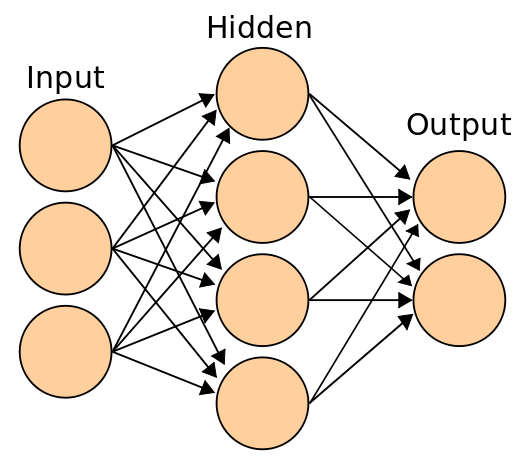
\includegraphics[width=6 cm]{images/ann.png}
        \caption{Minh họa cấu trúc của một mạng neural. \cite{ann_struct}}
        \label{fig:ann_structure}
    \end{figure}
    
    Ta có thể mô tả hoạt động mạng neural bằng công thức
    \begin{equation} \label{ann_eqn}
        y^{(l)}_i = f^{(l)}_i\left(\sum_{j=1}^{n^{(l-1)}}w^{(l)}_{ij}y^{(l-1)}_{j} + b^{(l)}_i\right).
    \end{equation}
    Trong đó:
    \begin{itemize}
        \item $l=1\dotsc L$, với $L$ là số lớp của mạng và $n^l$ là số neural ở lớp thứ $l$.
        \item $y^{(l)}_i$ là đầu ra của neural thứ $i$ ở lớp thứ $l$, với $i = 1\dotsc n^{l}$.
        \item $f^{(l)}_i$ là hàm truyền của neural thứ $i$ ở lớp thứ $l$. Hàm truyền tồn tại nhiều lựa chọn và mỗi lựa chọn có ảnh hưởng lớn đến kết quả đầu ra của mạng.
        \item $w_{i}^{(l)}$ là trọng số của đầu vào thứ $i$ ở lớp thứ $l$ thể hiện độ mạnh của từng đầu vào đối với quá trình xử lý thông tin để chuyển đổi dữ liệu từ lớp này sang lớp khác.
        \item Đầu vào của mạng là $y^{(0)} = \textbf{x}$ và đầu ra cuối là $\textbf{y} = y^{(L)}$.
        \item $b^{(l)}_i$ là \textit{ngưỡng} (bias) của neural thứ $i$ ở lớp thứ $l$.
    \end{itemize}
    
    Như vậy, quá trình học của mạng neural là quá trình tìm bộ trọng số $\textbf{w}$ sao cho phù hợp nhất. Quá trình này sẽ lặp liên tục và có thể không dừng đến khi tìm ra kết quả như ý. Vì vậy, trong thực tế, khi huấn luyện một mô hình mạng neural, một tiêu chuẩn dựa trên một giá trị sai số nào giữa đầu ra của mạng và đầu ra mong muốn cần được thiết lập, hoặc một số lần lặp tối đa xác định nào đó. Từ đây, ta tiếp cận thuật toán lan truyền ngược (Backpropagation), được sử dụng để điều chỉnh các trọng số liên kết sao cho tổng sai số nhỏ nhất. Với các mạng neural hiện đại, giải thuật được sử dụng kết hợp với một phương pháp tối ưu hóa như gradient descent để rút ngắn thời gian chạy của mạng.
    
    \subsubsection{Backpropagation}
    Trước hết, Gradient descent là một thuật toán tìm giá trị nhỏ nhất của hàm số f(x) dựa trên đạo hàm của nó. Thuật toán gồm 3 bước chính: (1) Khỏi tạo giá trị $x = x_0$ tùy ý; (2) Tính $x_1 = x_0 - \eta f'(x_0)$, với $\eta$ là \textit{learning rate} (tạm dịch là tốc độ học); (3) Tính lại $f(x)$ với các giá trị $x$ mới, sao cho nếu $f(x)$ đủ nhỏ thì dừng lại, còn không, lặp lại bước (2) với $x_2, x_3,\dotsc$
    
    Ta có thể nói, thuật toán lan truyền ngược áp dụng Stochastic Gradient Descent (gradient descent ngẫu nhiên - SGD) cho mạng neural có mục tiêu là tìm giá trị nhỏ nhất cho hàm $e(\textbf{w})$ qua đạo hàm $\nabla e(\textbf{w}): \dfrac{\partial e(\textbf{w})}{\partial w^{(l)}_{ij}}$ với toàn bộ $i, j, l$. Điểm khác biệt lớn của SGD là bước khởi tạo toàn bộ các trọng số sẽ khởi tạo ngẫu nhiên để tránh \textit{bias}.
    
    \subsubsection{Recurrent Neural Network (RNN)}
    Hình \ref{fig:ann_structure} ở phần trước là một ví dụ cho \textit{mạng neural nhân tạo truyền thẳng} (Feedforward Neural Network - FNN) gồm hai lớp ẩn kết nối hoàn toàn với nhau ở mỗi nút. Kiến trúc mạng truyền thẳng như trên không có các kết nối ngược trở lại từ các neural đầu ra về các neural đầu vào và mạng không lưu lại các giá trị output trước cũng như các trạng thái kích hoạt của neural. 
    
    Một kiểu kiến trúc khác là kiến trúc phản hồi (feedback), hay còn có tên là mạng neural hồi quy (Recurrent Neural Networ - RNN) cho phép đưa tín hiệu theo cả hai hướng thẳng và ngược lại bằng các vòng lặp. Mạng lưu lại các trạng thái trước đó, và hơn nữa, các trạng thái tiếp theo không chỉ phụ thuộc vào các tín hiệu đầu vào, mà còn phụ thuộc vào các trạng thái trước đó của mạng. Ý tưởng đằng sau RNN là RNN giống như trí nhớ ngắn hạn (Short Term Memory - STM) trong não người, tức là, RNN sẽ "học" và "ghi nhớ" lại thông tin ở chu kì trước và áp dụng ở bước "học" tiếp theo.
    \clearpage
    \begin{figure}[htp]
        \centering
        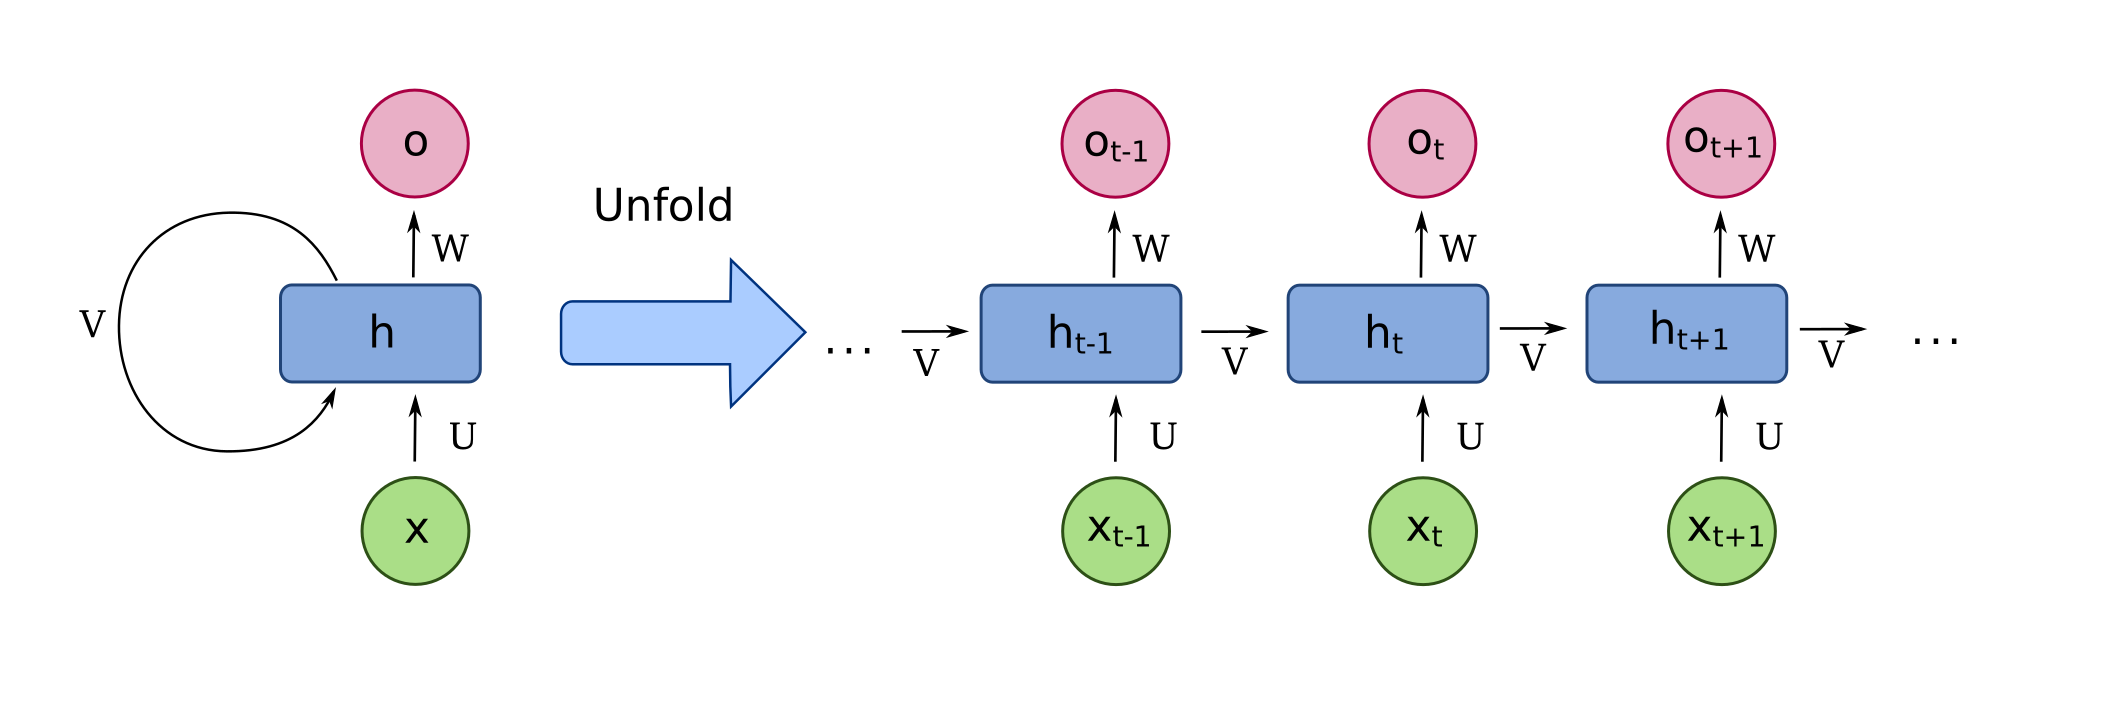
\includegraphics[width=15 cm]{images/rnn_unfold.png}
        \caption{Mô hình mạng neural hồi quy. \cite{rnn_unfold}}
        \label{fig:rnn_unfold}
    \end{figure}
    
    Dựa theo hình \ref{fig:rnn_unfold}, trong đó, $x_t$ và $o_t$ lần lượt là đầu vào và đầu ra tại thời điểm thứ $t$, $h_t$ là trạng thái ẩn tại thời điểm thứ $t$ và đóng vai trò là bộ nhớ của mạng. $h_t$ sẽ được tính dựa trên sự kết hợp giữa các trạng thái ẩn trước và đầu vào. Ta có thể viết:
    $$h_t = f(Ux_t + VS_{t-1}).$$
    
    Sau đó, $o_t$ sẽ được tính dựa theo $Wh_t$, với $(U, V, W)$ là ba tham số của mạng. Hai loại hàm truyền $f$ phổ biến nhất là hàm tanh hoặc hàm ReLU.
    
    Với khả năng “nhớ” được, mạng neural hồi quy được sử dụng để xử lý thông tin dạng chuỗi và các dữ liệu thời gian. Một số ứng dụng tiêu biểu là: mô hình ngôn ngữ và phát sinh văn bản, dịch máy (Machine Translation) và phát sinh mô tả cho ảnh (Generating Image Descriptions).
    
    \subsubsection{Hạn chế của RNN}
    Việc huấn luyện một RNN, cũng tương tự như mạng bình thường, sẽ sử dụng lan truyền ngược - Backpropagation như trên. Tuy nhiên, do bản chất có bộ nhớ của RNN, quá trình lan truyền ngược này sẽ được thực hiện qua từng thời điểm trong mạng. Quá trình này được gọi là \textit{lan truyền ngược liên hồi} (backpropagation through time).
    
    Mục tiêu là tính đạo hàm của lỗi với tham số $(U, V, W)$ tương ứng, sau đó, học các tham số này bằng cách sử dụng gradient descent. Ta có, ở từng trạng thái $h$, đạo hàm của hàm lỗi được khai triển như sau:
    $$\sum_t\dfrac{\partial e_t(\textbf{w})}{\partial\textbf{w}}\propto\sum_t\left(\prod_{i=k+1}\dfrac{\partial h_i}{\partial h_{i-1}}\right)\dfrac{\partial h_k}{\partial\textbf{w}}.$$
    
    Giả sử, trong trường hợp giá trị $\left\|\dfrac{\partial h_i}{\partial h_{i-1}}\right\|_2 < 1$, giá trị cập nhật sẽ bị giảm về gần 0 rất nhanh. Ví dụ, nếu lượng cập nhật chỉ là 0.01, nhưng qua 100 thời điểm, thì giá trị trên sẽ là $0.01^{100} \approx 0$. Mà khi đạo hàm bằng 0 thì có nghĩa là xảy ra hiện tượng bão hòa dẫn đến các nút phía trước cũng sẽ bị bão hoà theo. Vấn đề này không chỉ xảy ra với mạng RNN mà ngay cả mạng neural thường khá sâu cũng có hiện tượng này. Người ta gọi đây là hiện tượng \textbf{mất mát đạo hàm} (vanishing gradient).
    
    Một phương pháp phổ biến để giải quyết tình trạng mất mát đạo hàm là sử dụng kiến trúc mạng nhớ dài-ngắn hạn (Long Short-Term Memory (LSTM)). 
    
    \subsubsection{Long Short-Term Memory (LSTM)}
    \begin{figure}[htp]
        \centering
        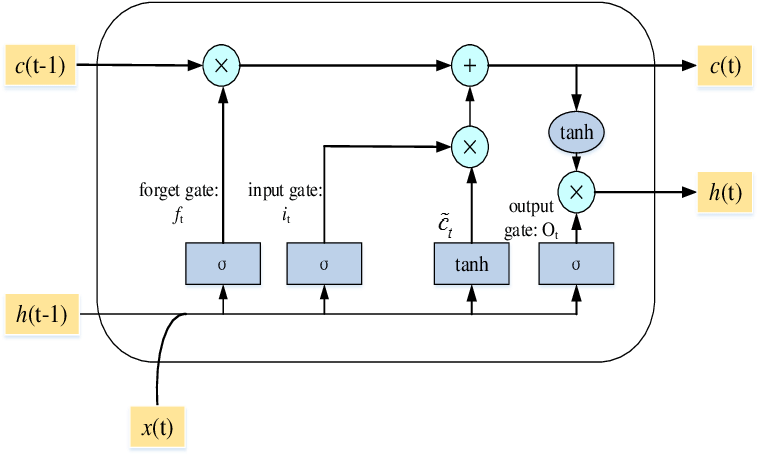
\includegraphics[width=14 cm]{images/lstm_struct.png}
        \caption{Cấu trúc của LSTM. \cite{lstm_struct}}
        \label{fig:lstm_struct}
    \end{figure}
    LSTM là một mô hình cải tiến của RNN và có cấu trúc tương tự nhưng khác ở cách tính toán đối với các trạng thái ẩn. Mấu chốt của khả năng “nhớ lâu” của LSTM là cấu trúc “trạng thái nhớ”. Ngoài ra, quá trình thêm hoặc loại bỏ thông tin sẽ dựa trên qui định của các cổng. Tóm lại, cốt lõi của mạng LSTM bao gồm trạng thái nhớ và các cổng.
    
    Các cổng của LSTM là một phương pháp định nghĩa thông tin băng qua và chúng được tạo bắng hàm sigmoid $\sigma$. Cụ thể, hàm sigmoid có giá trị thuộc khoảng (0, 1) mang ý nghĩa độ lớn thông tin được phép truyền qua tại mỗi lớp mạng. Nếu kết quả là 0,  điều này có nghĩa là không thông tin nào được phép đi qua, và ngươc lại, 1 nghĩa là toàn bộ thông tin được đi qua.
    
    Một mạng LSTM có 3 loại cổng, đều có đầu vào là trạng thái trước, đặt tên là $S \in \{h, c\}$, và đầu vào, nhân với trọng số tương ứng. Lưu ý, các cổng sẽ nhận một loại trọng sô khác nhau:
    \begin{itemize}
        \item \textbf{Cổng quên (Forget gate)} $f_t = \sigma(W_fS_{t-1} + W_fX_t)$.
        \item \textbf{Cổng vào (Input gate)} $i_t = \sigma(W_iS_{t-1} + W_iX_t)$
        \item \textbf{Cổng ra (Output gat)} $o_t = \sigma(W_oS_{t-1} + W_oX_t)$
    \end{itemize}
    
    Sau đó, trạng thái nhớ trung gian có thể được tính bằng hàm tanh qua công thức $\Tilde{C}_t = \text{tanh}(W_cS_{t-1} + W_cX_t)$. Từ đây, \textbf{trạng thái nhớ} sẽ nhận trạng thái trung gian và trạng thái nhớ trước, kết hợp với cổng vào và cổng quên như sau:
    \begin{equation} \label{lstm_cell_state_eqn}
        c_t = (i_t\times\Tilde{C}_t) + (f_t\times c_{t - 1}).
    \end{equation}
    
    Cuối cùng, trạng thái ẩn sẽ được tính bằng hàm tanh của trạng thái nhớ nhân với cổng ra:
    \begin{equation} \label{lstm_hidden_state_eqn}
        h_t = o_t\times\text{tanh}(c_t).
    \end{equation}
    
    Lưu ý, phép nhân trong công thức \ref{lstm_cell_state_eqn} và \ref{lstm_hidden_state_eqn} phụ thuộc vào $S$, tức là, các cổng sẽ thực hiện tính cho cả $h$ và $c$, sau đó, thực hiện phép nhân tương ứng cho mỗi loại trạng thái.